% Beamer template
% Author: Ozgur Taylan TURAN
% Delft University of Technology

\documentclass[aspectratio=169]{beamer}
% PACKAGES
\usepackage[english]{babel}
\usepackage{graphicx}
\usepackage{animate}
%\usepackage{calc}
\usepackage{calligra}
\usepackage[absolute,overlay]{textpos}
\usepackage[T1]{fontenc}
%\usefonttheme{serif}
\usefonttheme{professionalfonts}
\usepackage{amsmath}
\usepackage{palatino}
\usepackage{mathpazo}
\usepackage{graphicx}
%\usepackage{subfig}
\usepackage{tikz}
\usetikzlibrary{shapes,arrows}
\usepackage{xcolor}
\usepackage[T1]{fontenc}
%\usefonttheme{serif}
%\usepackage{titling}
\usepackage{graphicx}
\graphicspath{{Figures/}} %Setting the graphicspath
%\usepackage{subfig}
%\usepackage{tikz}
%\usetikzlibrary{shapes,arrows}
\usepackage{mathtools}
\usepackage{cancel}
\usepackage{tikz}
\usepackage{pgfplots}
% CUSTOM PACKAGES
\usepackage{/home/taylanot/texmf/tex/beamerthemetot}
\input{/home/taylanot/texmf/presentation/tune.tex}

 % COVER PAGE INFO   
\newcommand{\mytitle}{\color{White}\huge{\textbf{Lab Talk \#2}}}
\newcommand{\mysubtitle}{\color{Pink}\Large{\textbf{Expected Loss of Model-Agnostic Meta-Learning (MAML)}}}
\newcommand{\myauthor}{\color{White}\textcalligra{\LARGE Ozgur Taylan Turan}}
\newcommand{\authorlabel}{\small O.T. Turan}
\author{\authorlabel}


\begin{document}
% COVER PAGE

{
\def\beamer@entrycode{\vspace*{-\headheight}}
\setbeamertemplate{frametitle}[default][center]
\usebackgroundtemplate{\includegraphics[width=\paperwidth,height=\paperheight]{cover/coverart.pdf}}

\begin{frame}[plain] 

\begin{minipage}{\textwidth}
	\centering{\mytitle} \\
	\vspace{1cm}
	\centering{\color{White}\today} \\
	\vspace{1cm}
	\centering{\myauthor}\\
\end{minipage}


\end{frame}
}

\begin{frame}
	\centering
	\mysubtitle
\end{frame}

\section{Outline}
\begin{frame}
  \begin{itemize}
    \item How and Why did I ended up here?
    \item Learning-to-Learn
    \item MAML vs Biased Ridge
    \item Some Results/Conclusions
    \item What is next?
  \end{itemize}
\end{frame}

\section{How and Why?}
\begin{frame}{Constitutive Modeling}
\begin{minipage}{0.45\textwidth}
  \includegraphics<1>[width=\textwidth]{Figures/intro/scales.pdf} 
  \includegraphics<3>[width=\textwidth]{Figures/intro/link.png} 
\end{minipage}%
\begin{minipage}{0.55\textwidth}
  \color{Pink} Composite Materials  \color{Black}
  \begin{itemize}
    \item<1-3> Why?
    \item<1-3> How? \only<2>{\color{Pink} Experimental $\to$ time and money}
                    \only<3>{\color{Pink} Computational $\to$ time}
  \end{itemize}
\end{minipage}
\end{frame}

\begin{frame}{Computational Constitutive Modeling (Relationship between force and displacement}
\begin{minipage}{0.5\textwidth}

  \only<1-2>{\centering\color{Pink} Macro-scale Problem}
  \includegraphics<1-2>[width=\textwidth]{Figures/intro/link.png} 
  \only<3>
  {
    \begin{itemize}
      \item Inversion of a matrix (dof$\times$dof) at each step (\color{Pink} time\color{Black}) 
    \end{itemize}
  }
\end{minipage}%
\begin{minipage}{0.5\textwidth}
  \only<1-2>{\centering \color{Pink} Micro-scale Problem}

  \includegraphics<2>[width=0.8\textwidth]{Figures/intro/rve81.pdf} 

  \includegraphics<3>[width=0.8\textwidth]{Figures/intro/nonlinear.pdf} 
\end{minipage}
\end{frame}

\begin{frame}{Review}
\begin{minipage}{0.5\textwidth}
  \includegraphics[width=\textwidth]{Figures/FE2.pdf}
\end{minipage}%
\begin{minipage}{0.5\textwidth}
  \begin{itemize}
    \item Computationally model composites
    \item Time is the bottleneck of the model
  \end{itemize}
\end{minipage}
\end{frame}

\begin{frame}{Machine Learning to the Rescue}
\begin{minipage}{0.5\textwidth}
  \includegraphics<1>[width=\textwidth]{Figures/FE2.pdf}
\end{minipage}%
\begin{minipage}{0.5\textwidth}
  \includegraphics<1>[width=\textwidth]{Figures/FE2-ML.pdf}
\end{minipage}
\end{frame}

\begin{frame}{Machine Learning to the Rescue}
\begin{minipage}{0.5\textwidth}
  \begin{itemize}
    \item $\mathbf{P}^\Omega=\mathcal{C}(\mathbf{F}^\Omega, \{c\}_{i=1}^t)$
    \item Current Appplication: Focus on one curve to create a surrogate
    \item Why not consider other curves that might come from some other source!
  \end{itemize}
\end{minipage}%
\begin{minipage}{0.5\textwidth}
  \includegraphics<1>[width=\textwidth]{Figures/example.pdf}
\end{minipage}
\end{frame}

\section{Learning-to-Learn}

\begin{frame}{Learning-to-Learn Intro}
\begin{minipage}{0.5\textwidth}
  \color{Pink} Learning \color{Black}
  \begin{itemize}
    \item<1> Task $\to$ $f:\mathbf{x}\mapsto y$
    \item<1> Training experience $\to$ $\mathcal{Z}=\{\mathbf{x}_i,y_i\}_{i=0}^N$
    \item<1> Error measure $\to$ $\mathcal{L}:=\sum_j^M(\mathcal{M}_j-y_j)^2$
  \end{itemize}
\end{minipage}%
\begin{minipage}{0.5\textwidth}
  \color{Pink} Learning-to-learn \color{Black}
  \begin{itemize}
    \item<2> Family of Tasks $\to$ $\{f_k:\mathbf{x}\mapsto y\}_{k=1}^{K}$
    \item<2> Training experience for $f_k$ $\to$ $\mathcal{Z}_k$
    \item<2> Error measure for each task $\to$ $\mathcal{L}_k$
  \end{itemize}
\end{minipage}
  \begin{itemize}
  \centering
    \item<3> Learning a function vs learning a functional (space of functions!)
  \end{itemize}
\end{frame}

\begin{frame}{Learning-to-learn Intro}
  \centering
  \includegraphics[width=0.75\textwidth]{singlevsmeta}
\end{frame}

\begin{frame}{Learning-to-learn}
  \begin{itemize}
    \item since 90's 
    \item rooted with LSTM type of meta-learners 
    \item Now, gradient descent based adaptation based NN's $\to$ $MAML$
  \end{itemize}
\end{frame}


\begin{frame}{Questions?}
  \begin{itemize}
      \item Does the claims for generalization hold?
      \item Can this framework outperform a single-task learner in expectation?
  \end{itemize}
\end{frame}

\section{MAML vs Biased Ridge}
\begin{frame}{Problem Setting-1}
  \begin{minipage}{0.5\textwidth}
    \color{Pink} Linear Problem \color{Black}
    \begin{itemize}
      \item<1> $ \mathbf{a} \in \mathbb{R}^d \to p_\mathcal{T} \sim \mathcal{N}(m\mathbf{1},c\mathbf{I})$
      \item<1>$ \mathbf{x} \in \mathbb{R}^d \to p_\mathbf{x} \sim \mathcal{N}(\mathbf{0},k\mathbf{1})$
      \item<1>$ \varepsilon \sim \mathcal{N}(0,\sigma^2)$
      \item<1>$ y = \mathbf{a}^\text{T}\mathbf{x} + \varepsilon \quad \in \mathbb{R}$
      \item<1>$ \mathcal{Z}:= ((x_i,y_i))_{i=1}^N$
      \item<1>$ \hat{\mathcal{M}} \to $ an estimator trained with $\mathcal{Z}$
    \end{itemize}
  \end{minipage}%
  \begin{minipage}{0.5\textwidth}
    \includegraphics<1>[width=0.9\textwidth]{lintask}
  \end{minipage}

\dotfill

  \color{Pink} Expected Error for an estimator: \color{Black}
  \centering
  $ \mathcal{E}:=\int \int \int (\hat{\mathcal{M}}-y)^2p(x,y)dxdyp_\mathcal{Z}d\mathcal{Z}p_\mathcal{T}d\mathcal{T}$
\end{frame}

\begin{frame}{Problem Setting-2}
  \begin{minipage}{0.5\textwidth}
    \includegraphics<1>[width=0.9\textwidth]{nonlintask}
  \end{minipage}%
  \begin{minipage}{0.5\textwidth}
     \color{Pink} Nonlinear Problem \color{Black}
    \begin{itemize}
      \item<1> $ \mathbf{a} \in \mathbb{R}^d \to p_\mathbf{a} \sim \mathcal{N}(\mathbf{1},c_1\mathbf{I})$
      \item<1> $ \boldsymbol{\phi} \in \mathbb{R}^d \to p_{\boldsymbol{\phi}} \sim \mathcal{N}(\mathbf{0},c_2\mathbf{I})$
      \item<1> $ \mathbf{x} \in \mathbb{R}^d \to p_x \sim \mathcal{N}(\mathbf{0},k\mathbf{1})$
      \item<1> $ \varepsilon \sim \mathcal{N}(0,\sigma^2)$
      \item<1> $ y = \mathbf{a}^\text{T}\text{sin}(\mathbf{x}+\phi) + \varepsilon \quad \in \mathbb{R}$
      \item<1> $ \mathcal{Z}:= ((x_i,y_i))_{i=1}^N$
      \item<1> $ \hat{\mathcal{M}} \to $ an estimator trained with $N$ training points
    \end{itemize}
  \end{minipage}

\dotfill

  \color{Pink} Expected Error for an estimator: \color{Black}
  \centering
  $ \mathcal{E}:=\int \int \int (\hat{\mathcal{M}}-y)^2p(x,y)dxdyp_\mathcal{Z}d\mathcal{Z}p_\mathcal{T}d\mathcal{T}$
\end{frame}

\begin{frame}{Models}
  \begin{block}{\color{White} Problem Setting-1}
  \begin{itemize}
    \item Linear Model $\to$ Least-Squares and Gradient Descent
    \item Ridge $\to$ with bias and without bias
    \item MAML
  \end{itemize}
  \end{block}

 \begin{block}{\color{White} Problem Setting-2}
  \begin{itemize}
    \item Kernel Ridge
    \item MAML
  \end{itemize}
  \end{block}
\end{frame}

\begin{frame}{MAML\cite{Finn2017}}
\begin{minipage}{0.5\textwidth}
  \includegraphics<1>[width=\textwidth]{maml}
\end{minipage}%
\begin{minipage}{0.5\textwidth}
  \begin{itemize}
    \item<1> Sample Tasks 
    \item<1> Sample training experiences from that tasks
    \item<1> Check the possible loses 
    \item<1> Take average step
  \end{itemize}
\end{minipage}
\centering
  \only<1> {For a model $\mathcal{M}$ parametrized by $(\mathbf{w})$}
\end{frame}

\begin{frame}{MAML\cite{Finn2017}}
  \begin{minipage}{0.5\textwidth}
    \includegraphics<1>[width=\textwidth]{maml_linear}
  \end{minipage}%
  \begin{minipage}{0.5\textwidth}
    \includegraphics<1>[width=\textwidth]{maml_nonlinear}
  \end{minipage}
\end{frame}

\begin{frame}{Biased Ridge\cite{Denevi2018a}}
\begin{minipage}{0.5\textwidth}
  \includegraphics<1>[width=0.95\textwidth]{ridge}
\end{minipage}%
\begin{minipage}{0.5\textwidth}
  \begin{itemize}
    \item<1> Sample Tasks 
    \item<1> Sample training experiences from that tasks
    \item<1> adjust the bias
  \end{itemize}
\end{minipage}
\centering
  \only<1>{ For a model $\mathcal{M}$ parametrized by $(\mathbf{w})$ minimize $\mathcal{L}+\lambda||\mathbf{w}-\mathbf{h}||^2_2$}

\end{frame}

\section{Results/Conclusions}
\begin{frame}{Problem Setting-1}
  \centering
  \only<1>{
  Limit the number of gradient steps for adaptation to 1 and other parameters regarding the problem is defaulted to 1 as well.
  }

  \begin{minipage}{0.5\textwidth}
    \centering
    \includegraphics<1>[width=0.8\textwidth]{c_1_1}

    \only<1>{N=1}
  \end{minipage}%
  \begin{minipage}{0.5\textwidth}
    \centering
    \includegraphics<1>[width=0.8\textwidth]{c_1_10}

    \only<1>{N=10}
  \end{minipage}

  \only<2>{


    \color{Pink} Only consider the $c=[0,1]$ \color{Black}
  \begin{tabular}{c|c|c|c|c|c|c|c|c|c|c|c|}
    \cline{2-11}
     & \multicolumn{10}{|c|}{number of gradient steps}\\
    \cline{2-11}
     & 1 & 2 & 3 & 4 & 5 & 6 & 7 & 8 & 9 & 10\\
    \hline
    \multicolumn{1}{|c|}{MAML} & 1.21& \textbf{1.19} & 1.20& 1.21& 1.23& 1.24& 1.27& 1.33& 1.46& 1.75\\
    \hline
  \end{tabular}

  }
\end{frame}

\begin{frame}{Problem Setting-2}
  Every other parameter is defaulted to 1, and the adaptation steps used is 5.
  \begin{minipage}{0.33\textwidth}
    \centering
    \includegraphics<1>[width=\textwidth]{c2_1_1}
    N=1
  \end{minipage}%
  \begin{minipage}{0.33\textwidth}
    \centering
    \includegraphics<1>[width=\textwidth]{c2_1_10}
    N=10
  \end{minipage}%
  \begin{minipage}{0.33\textwidth}
    \centering
    \includegraphics<1>[width=\textwidth]{c2_1_50}
    N=50
  \end{minipage}%
\end{frame}

\begin{frame}{Conclusions}
  \begin{minipage}{0.5\textwidth}
    \begin{itemize}
      \item<1> Benefit of MAML only for $p_\mathcal{T}$ with small variance...
      \item<2> Number of gradient steps taken is a clear regularizing effect...
      \item<2> Not, a huge gain though???
    \end{itemize}
  \end{minipage}%
  \begin{minipage}{0.5\textwidth}
    \includegraphics<1>[width=\textwidth]{task_variance}
  \end{minipage}
\end{frame}


\begin{frame}{So, the question is...}
  \begin{itemize}
    \item Can we come up with a meta kernel ridge model that can outperform MAML?
    \item I think yes we, can
  \end{itemize}
\end{frame}

\begin{frame}{Remember Kernel Ridge}
Thanks to Nonparameteric Representer Theorem for $g\to\mathbb{R}$ be strictly increasing and $\mathcal{L}$ being a loss function that is monotonic, then $${min}_{f\in\mathcal{H}}\quad\mathcal{L} + g(||f||_\mathcal{H})$$  has the solution in the form, $$f(\cdot)=\sum^N_i\alpha_i k(\cdot,\mathbf{x}_i).$$ 
$\mathcal{L}=\sum_i^N(f(\mathbf{x}_i)-y_i)^2$.
 For $g(||f||_\mathcal{H}):=\lambda||f||^2$, the optimal solution is given by:
	$$\boldsymbol{\alpha}=(\mathbf{K}+\lambda \mathbf{I})^{-1}\mathbf{y}$$
\end{frame}

\begin{frame}{Semiparametric Kernel Ridge}
In the Semiparameteric Representer Theorem  $\tilde{f}:= f + h$ where $h\in span\{\psi_p\}$ where $\{\psi_p\}_{p=1}^M$ are real valued functions and $\mathcal{L}=\sum_i^N(\tilde{f}(\mathbf{x}_i)-y_i)^2$. Then the solution to 
 $${min}_{f\in\mathcal{H}}\quad\mathcal{L} + g(||f||_\mathcal{H})$$  has the form $$f(\cdot)=\sum^N_i\alpha_i k(\cdot,\mathbf{x}_i)+\sum_j^M\beta_j\psi_j(\cdot).$$ 
 For $g(||f||_\mathcal{H}):=\lambda||f||^2$, the optimal solution is given by:
	$$\boldsymbol{\alpha}=(\mathbf{K}+\lambda\mathbf{I})^{-1}(\mathbf{y}-\boldsymbol{\psi}\boldsymbol{\beta})$$   
  $$\boldsymbol{\beta}=\boldsymbol{\psi}^{-1}(\mathbf{y}-\mathbf{K}\boldsymbol{\alpha})$$
\end{frame}

\begin{frame}{Simple Example Case}
  \begin{minipage}{0.45\textwidth}
  \begin{itemize}
    \item Consider the Problem Setting-2
    \item Assume 10 ground-truth tasks are provided as for $D=1$ $\psi(x)=\mathbf{a}^\text{T}\text{sin}(\mathbf{x}+\phi)$
  \end{itemize}
  \end{minipage}%
  \begin{minipage}{0.55\textwidth}
    % This file was created with tikzplotlib v0.10.1.
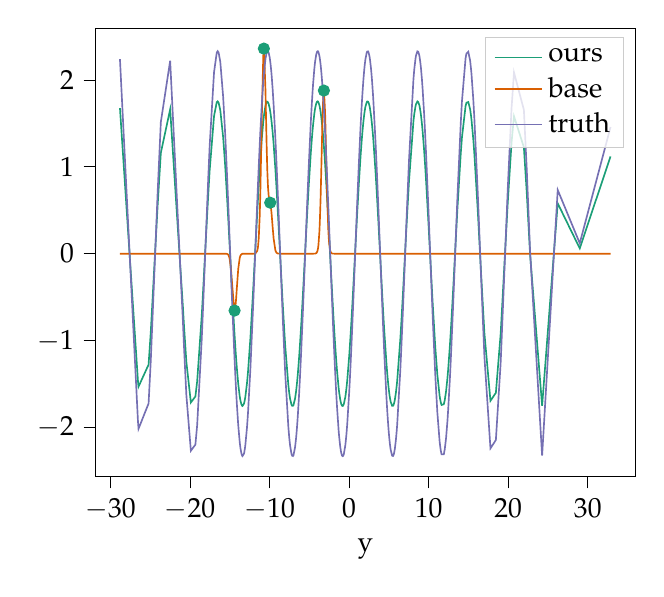
\begin{tikzpicture}

\definecolor{chocolate217952}{RGB}{217,95,2}
\definecolor{darkcyan27158119}{RGB}{27,158,119}
\definecolor{darkgray176}{RGB}{176,176,176}
\definecolor{lightgray204}{RGB}{204,204,204}
\definecolor{lightslategray117112179}{RGB}{117,112,179}

\begin{axis}[
legend cell align={left},
legend style={fill opacity=0.8, draw opacity=1, text opacity=1, draw=lightgray204},
tick align=outside,
tick pos=left,
x grid style={darkgray176},
xlabel={y},
xmin=-31.8753828186506, xmax=35.94436113938,
xtick style={color=black},
y grid style={darkgray176},
ymin=-2.5635714926033, ymax=2.59329741951645,
ytick style={color=black}
]
\addplot [draw=darkcyan27158119, fill=darkcyan27158119, forget plot, mark=*, only marks]
table{%
x  y
-14.387132798348 -0.654614863946559
-10.7081625562024 2.35889428714737
-9.90810386640961 0.586437105942268
-3.1628035962143 1.87616747303034
};
\addplot [semithick, darkcyan27158119]
table {%
-28.7926671841947 1.67438847182915
-26.5319553194153 -1.46381251924785
-26.4598660796463 -1.52936780592978
-25.1952444826706 -1.27621070127736
-24.9171125752942 -0.897547744453766
-24.2073761024031 0.299753971757634
-24.0526504326644 0.562212847698647
-23.6557181958013 1.16004570122924
-22.4836144318131 1.66047816532522
-20.8829183428752 -0.60868125482829
-20.789010136596 -0.760065312965487
-20.753896568733 -0.815019203938319
-20.4508172604874 -1.24079772183709
-19.8827031028175 -1.71150281845736
-19.3113743086402 -1.64256024731714
-19.0888070712066 -1.46741689376146
-18.5184940243225 -0.718256913519847
-18.4375125826408 -0.586623515663498
-18.4037013409152 -0.530475836171671
-18.3069051615065 -0.366604312742437
-18.2914824320977 -0.340137106221981
-18.2732924480736 -0.308817472053943
-18.147233210844 -0.0895267212880879
-17.6909129315957 0.690701832065178
-17.5180743453447 0.957341534339633
-17.515485259906 0.961137746756199
-16.9691504721535 1.58238029742161
-16.6282858988335 1.74285974126971
-16.5141176391698 1.75202987580526
-16.3968664327789 1.73770445809758
-16.1821659266039 1.64998738183919
-15.8253819942168 1.34018157648471
-15.6016507671223 1.05636147711123
-15.5359408706782 0.962293456059405
-15.3359416760642 0.652231109229208
-15.2250603448742 0.468321732740854
-15.1867147743182 0.403280643562114
-15.1500328535812 0.340516582358783
-15.1364274505478 0.317119716103143
-15.0525112835388 0.171734138554456
-15.0176355070622 0.110932239894161
-14.86945803262 -0.147679610713393
-14.8172326079891 -0.238199191976733
-14.8111518828462 -0.248696026909653
-14.7405372421286 -0.369752326209966
-14.4318588437597 -0.86963844681082
-14.4027273879039 -0.913433575472654
-14.2800361408725 -1.08948059443501
-14.1941805535906 -1.20349933075539
-14.1435441461787 -1.26673110863449
-14.1275215259523 -1.28607635492788
-14.1053743792435 -1.31227270028923
-13.9294080642568 -1.49631275265784
-13.9284187779294 -1.49721938134909
-13.7366161489579 -1.64380877562889
-13.6469549346657 -1.69162187357835
-13.5260040882223 -1.73438616049974
-13.4334784405776 -1.74995447563012
-13.3973228326511 -1.75196672122054
-13.2110519378543 -1.72608245284517
-13.1716442677356 -1.7128822050608
-13.0857001181078 -1.67490170828497
-13.0369764674579 -1.64785626234718
-12.8312682143741 -1.49148644319194
-12.7990816442036 -1.46112381601088
-12.6994742105633 -1.3577191095459
-12.6932837209066 -1.35083706895333
-12.6816223516761 -1.33773259313711
-12.4043716553613 -0.976920223504369
-12.0578490531364 -0.424854842746269
-12.0264296988728 -0.371245625267336
-11.9841057217254 -0.29846072870041
-11.8897078575164 -0.134391140974736
-11.8690023149202 -0.0981919827955042
-11.7765868612864 0.0636754178990674
-11.534259716306 0.482171312482214
-11.4710188929985 0.587841180261994
-11.4358731686223 0.645625236673095
-11.3489572608752 0.785168057922256
-11.2293065525276 0.968088428563138
-11.1525359791087 1.07889500477523
-10.9481991176831 1.34300642201587
-10.7803946410402 1.51780929393755
-10.69197832855 1.59143082936168
-10.6898689845616 1.59301954047625
-10.6880020421607 1.59441904323782
-10.5096764777657 1.69880565838819
-10.4999708690417 1.70280653803792
-10.4960983676342 1.70435436366221
-10.3917763273463 1.73568502992038
-10.3587270384876 1.74147358751854
-10.3550115666475 1.74200113906115
-10.298285865801 1.74699058391306
-10.2656335018412 1.7472812729175
-10.1879181581497 1.74056476285936
-10.1015801942666 1.72131180866333
-9.98815115887008 1.67832231291483
-9.9222289958395 1.64466540961
-9.86977140040626 1.61351349961936
-9.78665665648765 1.55634597762334
-9.76805045814489 1.5422364012593
-9.72703105495225 1.50942269552626
-9.60924474608834 1.40198194649165
-9.48726113631224 1.26994026949263
-9.48296936193739 1.26491609882231
-9.26610005159563 0.980307649116205
-9.22622655898017 0.922079664572044
-9.21335758228762 0.902947018096406
-9.12796153683555 0.772133530366522
-8.96179770987439 0.501731061068667
-8.81856978050392 0.257029468330155
-8.81227234189458 0.246110763008704
-8.79462772736772 0.215466984198946
-8.73702727909187 0.115011614131585
-8.66791145124438 -0.0060038896069301
-8.6141509497351 -0.100144487164791
-8.59253080105267 -0.137937574486027
-8.57207642782401 -0.173633810715947
-8.46564009599612 -0.357874167770702
-8.40849973084543 -0.455244044867006
-8.36479368514026 -0.528734871778984
-8.35900900863911 -0.538389035816973
-8.32131507466745 -0.600841545193822
-8.09916220990386 -0.94871714535854
-8.06629739123137 -0.996608240167334
-8.01421681051039 -1.0702762924129
-7.63356970616655 -1.50906896460831
-7.52738225550011 -1.59493432075523
-7.48326994324296 -1.62537066446325
-7.47676972556646 -1.62958966484924
-7.40992639809723 -1.66894974643585
-7.40599630135363 -1.67103347892686
-7.40250769071922 -1.67286151305751
-7.24304435444085 -1.73437935268124
-7.2095105601884 -1.74174731381016
-7.15252543706475 -1.74977285422376
-7.04601592096298 -1.74953589692612
-7.02660233431039 -1.74735256523559
-6.98465157675271 -1.7403870219669
-6.7941182813103 -1.67052293386282
-6.66781734697402 -1.59063974752274
-6.64441854573807 -1.57301360244763
-6.60865100427492 -1.54440924714328
-6.53779469770057 -1.48194777046847
-6.47897845275925 -1.42443631877194
-6.43420540409313 -1.37734295851013
-6.32835674735168 -1.25521264730186
-6.27521137287909 -1.1885023396574
-6.26030533789618 -1.16918065505123
-6.18116791097957 -1.06235529383136
-6.09143706615567 -0.933223494026619
-6.06015011404703 -0.886377919205511
-6.05279675156811 -0.875240187990359
-6.01340297048143 -0.814781723926778
-6.00321911236443 -0.798942863606212
-5.98741977641202 -0.774206914405582
-5.97460159404949 -0.753996072246376
-5.95081863599867 -0.716171071085664
-5.8983971875738 -0.631398981835884
-5.88424302439267 -0.608202658644047
-5.86559635801841 -0.577458629261406
-5.78819932109669 -0.447823836599742
-5.78312890119562 -0.439229107367036
-5.75259028538142 -0.387232965228705
-5.72699985307231 -0.343381668109122
-5.60173630148088 -0.126030441065666
-5.55483320782477 -0.0439539835983795
-5.50644146858232 0.0408268017900132
-5.46104173539395 0.120282500043643
-5.41414297523025 0.202099522771909
-5.36628470758679 0.285131022531877
-5.32931815416325 0.348828857635034
-5.24691940727079 0.488969289681998
-5.07393619664919 0.771271623260685
-4.813762496399 1.15003227945742
-4.80828155061975 1.15726023159824
-4.74211192136967 1.24171539785353
-4.69118858917574 1.30302886339236
-4.5790360445319 1.42593960116173
-4.56971552212403 1.43536750262159
-4.52317084625647 1.48056636337556
-4.37129918560494 1.60527883964753
-4.30368260647988 1.64905654148146
-4.29583122478886 1.6536551004875
-4.29371324048122 1.65487816585784
-4.24935032436732 1.67878288033041
-4.12503471680907 1.72806448042473
-4.09485422139078 1.73603377001366
-4.00915589366006 1.75006264044036
-3.9742997984888 1.75212100095582
-3.90639280847082 1.75008366172608
-3.89207253106365 1.7486373926889
-3.86149455848401 1.74437036060328
-3.84982411635898 1.74231993048188
-3.73094854881308 1.7083251656742
-3.69222640912634 1.69217972150041
-3.67430211726768 1.68387779700559
-3.58856463973948 1.63702974827312
-3.56902349213582 1.62472144323223
-3.48207896507483 1.56274790934542
-3.47817131565783 1.55968840108614
-3.47395070089064 1.55635753056215
-3.38449382744645 1.47936313809292
-3.3494125568813 1.44585748257596
-3.29718536474684 1.39255675160486
-3.24074358632665 1.33041591787786
-3.21045568070522 1.29516164265584
-3.17224517503185 1.24882940309852
-3.16999112283568 1.2460326560501
-3.14867440430453 1.21923937992695
-3.00871763819469 1.02877858656846
-2.97846546164804 0.984581208245008
-2.87822785078684 0.831654206597791
-2.79292067740613 0.694895316425434
-2.78495200686086 0.681860730498705
-2.78269112502597 0.678155201364159
-2.76868900220007 0.655135600630535
-2.59912970030087 0.368505218010092
-2.56748055060031 0.313782849862429
-2.55303979545813 0.288725260955317
-2.53783085527012 0.262281539106819
-2.5178379250709 0.227445941157227
-2.49708575100603 0.191210775244604
-2.4937605254541 0.18539828346696
-2.36594403976095 -0.038690904024632
-2.33180876111982 -0.0985154461924942
-2.29948576787846 -0.155043120409934
-2.23340545251079 -0.270004776120687
-2.22317184925398 -0.287712631033473
-2.20438348842227 -0.320141992324227
-2.18777665286225 -0.348710799528108
-2.09600818933533 -0.504617214234613
-2.03753266072935 -0.601820006832062
-1.97131540858812 -0.709387183051844
-1.93990361775035 -0.759354760417014
-1.9270673682866 -0.779560798225992
-1.85985798647503 -0.883184524997679
-1.8272564131114 -0.932041494231822
-1.82346984190807 -0.937652851038619
-1.78257464652872 -0.997382519168438
-1.77610790632399 -1.00667735469272
-1.77399171527709 -1.00970989472741
-1.67094324581937 -1.15165284155783
-1.65339878374631 -1.17464167483377
-1.63771524741257 -1.19488624723981
-1.5742019523629 -1.27381455079478
-1.56736753714553 -1.28200705427938
-1.54659077731538 -1.30654312288401
-1.51767159182551 -1.33975380801124
-1.31960078173773 -1.53575754768771
-1.28491941146563 -1.5640808892421
-1.25157059418093 -1.58954230404217
-1.24305608138383 -1.59576084642134
-1.11323064081448 -1.67600476195873
-1.02091297122489 -1.71596451957151
-0.97755058769108 -1.729705776651
-0.918875598945228 -1.74311851799949
-0.88926870563566 -1.74761116982898
-0.861839050582677 -1.75040654196854
-0.806896394274196 -1.75204395633886
-0.747074670288275 -1.74781429518507
-0.671641819284936 -1.73357149773352
-0.667249690100152 -1.73243738503022
-0.658695006580819 -1.73013252099852
-0.477101792922125 -1.65168954712746
-0.42039006775422 -1.61589057953673
-0.341023565132514 -1.55709631162624
-0.330409702987032 -1.54848163282907
-0.306978166705565 -1.52884734286259
-0.278462465903734 -1.50382160315123
-0.225142629509054 -1.45376331029256
0.0220643462694602 -1.17024464952847
0.0633258873952078 -1.11545716202673
0.0934198706277455 -1.07429515557904
0.190223618488186 -0.935483320304192
0.203678348632758 -0.91546596264125
0.254952820865954 -0.837694373361386
0.257359464708347 -0.833988328643998
0.285169949895258 -0.79081742101283
0.369336751791834 -0.656576633581658
0.405470032024726 -0.597463424494921
0.480422504515399 -0.472445203025586
0.544014378063144 -0.364267606960091
0.632526045259428 -0.211343372846743
0.680896518880839 -0.126995948444746
0.769555966046685 0.0282351174164308
0.851521000440185 0.171575143791767
0.854711466151256 0.177137536686512
0.872009137341414 0.207262188096305
0.981823840826113 0.396689746264457
1.0200299291679 0.461588556382738
1.03149228304346 0.48093200154602
1.22103427885246 0.78975871856697
1.23069048147156 0.804824518259854
1.41421205753391 1.0753339219385
1.44010369899036 1.11078664303132
1.47306286894904 1.1548364423077
1.50015621595142 1.19010928786847
1.51479812920863 1.20880962296666
1.58533002647954 1.29519079159804
1.60774248304354 1.32131070005027
1.61172047363532 1.32587774428407
1.66613436390677 1.38621266553837
1.69395250164649 1.41548347335627
1.80285554061724 1.519336412448
1.82097038907104 1.53489515594714
1.90216730579767 1.59837738171068
1.95564409029754 1.63445779410886
2.03034997027372 1.67701706411151
2.03337115027604 1.67854281004638
2.03628240802988 1.67999854865988
2.06412214492131 1.69319861573907
2.21425903626525 1.74155428226014
2.2411960260881 1.74610206790077
2.28156830791583 1.75054505305248
2.38618859633228 1.74877850801661
2.44670491821762 1.73901655935326
2.55932157355923 1.70394654705115
2.56341370510596 1.70226221381831
2.59178042283747 1.68980430281617
2.640923517522 1.66501026238351
2.75746262045979 1.59027069720254
2.7651387829325 1.58457770377855
2.80420156047217 1.55416773218084
2.81856226251407 1.54238939822269
2.88740854409602 1.48155008975988
3.00033657188577 1.36670290259544
3.03555653158345 1.32724776232466
3.05841554693426 1.30075585933341
3.3428485746837 0.919082282455883
3.42211622904024 0.798073568082391
3.48012510452338 0.706297875805447
3.56128886841732 0.573971410375827
3.66424679165161 0.400790105141031
3.71398778384255 0.315486916228173
3.72181816029925 0.301981706513412
3.75322706637111 0.247632407148964
3.79461734906329 0.175647203733283
3.90853162028307 -0.0236502726569089
3.92537332049354 -0.0531518486100501
4.02567747653511 -0.228256302579599
4.08838188141401 -0.336666963725593
4.10319726132059 -0.362103996092444
4.26099707786335 -0.627002246695489
4.26440097688554 -0.63256776314194
4.30888273350407 -0.704599865800158
4.34079476917848 -0.755426469129896
4.34629806622393 -0.764115287084841
4.36224839572065 -0.789166608901458
4.36432248892389 -0.792409529432219
4.37109007698963 -0.802967120003479
4.4182027298657 -0.875418369127592
4.69520601653911 -1.25711900775466
4.7404571921626 -1.31104282984914
4.74099215642222 -1.31166448163578
4.75806663766795 -1.33130762437926
4.75827373767939 -1.33154350936471
4.79389786159366 -1.37126073557693
4.86077806321014 -1.44108729574288
4.91721612013254 -1.49501050943742
4.9843186416808 -1.55291480965846
4.98807330383821 -1.55595057321101
5.06474783004471 -1.61308856880659
5.06595038557392 -1.61391002328836
5.10736307594478 -1.64076665338598
5.13384540932594 -1.65646861427513
5.20933334223808 -1.6948181710231
5.22685171950128 -1.70234473180806
5.41121525601979 -1.74952736755258
5.52678248165144 -1.7488859806756
5.56596502386818 -1.74336268966072
5.6092136240917 -1.73415952938968
5.61463444386493 -1.73277685200546
5.66525322140358 -1.71741400299198
5.70481421732493 -1.70234193778054
5.72729785953189 -1.69258714901736
5.76490713579737 -1.6743600133392
5.89180824890819 -1.59555943596283
5.99421786725673 -1.51318425626909
6.03821743619573 -1.47286627406347
6.04934551383771 -1.46221441286322
6.43746661433901 -0.988116477241142
6.51931540097234 -0.866510864896188
6.58873789967718 -0.758786645729648
6.61660751170548 -0.714482778291087
6.76690181308148 -0.466884868737056
6.80302974087687 -0.405580987282199
6.86987824032483 -0.290813206137006
6.89340419769737 -0.250087455787417
6.89738202348755 -0.243187149360383
6.90000394410299 -0.238636811265823
6.92529166480381 -0.194670441854514
7.05489161173929 0.0320022536831073
7.06085203935571 0.042443383701459
7.0863513274163 0.0870899526954556
7.19600625088196 0.278075825417626
7.52910687339345 0.82843527567638
8.09444878400114 1.52662025490736
8.17171819377161 1.58844283960652
8.20375725311269 1.61131610199261
8.34183318939922 1.69070636077646
8.38853392660993 1.71033276927563
8.41501581238835 1.71980740934426
8.58524907530227 1.75170909310102
8.6973272440751 1.74506337174937
8.82819377467154 1.7096132424616
8.86080498589612 1.69619393358225
8.97439879819633 1.63547603870972
8.98184472738639 1.63074979574393
9.01463455134741 1.60886462914265
9.01637409800237 1.60765505985167
9.05172489598421 1.58202564451844
9.15888135123629 1.49240427950009
9.23076030566422 1.42262257386149
9.25134233976675 1.4012712490048
9.42286796272939 1.20116887370388
9.44713445583634 1.16986362576323
9.45849838675342 1.15496549878132
9.47312726440486 1.13556771331387
9.5502635823171 1.02936655214756
9.63768094975008 0.901645966041505
9.66854693607909 0.854852623594271
9.69700197102548 0.810991851111142
9.94987999542821 0.396613568116878
9.99620986557415 0.317146891363603
10.3372697530649 -0.277506400530172
10.3591774201452 -0.315337573800411
10.3989922565356 -0.383691607915905
10.4062924232351 -0.396161728804778
10.4353400492941 -0.445565132133823
10.4610943490853 -0.489054237253772
10.5176403151731 -0.58336070701466
10.792807221625 -1.01032320528145
10.8514927894722 -1.09254510426662
10.8553161722466 -1.09777435756928
11.0853775015119 -1.38026013545927
11.0973938404569 -1.39312933910712
11.3798278721687 -1.63408239958123
11.4438802018372 -1.67120231281046
11.5350094461074 -1.71217014555212
11.5695750851693 -1.7240071351003
11.573362864105 -1.72517927585124
11.6311525286575 -1.73998391656257
11.8992941146904 -1.73239197966235
11.9176586133655 -1.72728275081367
12.0220653259656 -1.68722787104028
12.1897247054663 -1.58472126823473
12.3641782573812 -1.43093610823118
12.468082197083 -1.31834575500349
12.6699744905308 -1.06014345254423
12.7728776602552 -0.911236345672196
12.7736308788231 -0.91010886300366
12.7946132527021 -0.878495407240519
12.8596300808563 -0.77814354465714
13.0698024753304 -0.433501191944203
13.0962451103043 -0.388464109102209
13.1364946015171 -0.319400420668894
13.1814395587357 -0.241673583280479
13.2048323352675 -0.201015511047464
13.2981433011935 -0.0379622768058798
13.3393983998568 0.0343172581641077
13.4250032692548 0.183971427272682
13.4805649867833 0.280451501877867
13.6301882156987 0.535134378377567
14.0417135147095 1.15783784691091
14.1878926203614 1.33704098338611
14.6437674748202 1.69903131355816
14.7577385420919 1.73669624311866
14.984068989869 1.74449285940347
15.2077833878009 1.66474310028065
15.2324442714655 1.65076196144436
15.2324767231215 1.65074290012856
15.3411300773681 1.57731076555947
15.3894538246965 1.53861546868306
15.6068099568483 1.32164672850945
15.6221994442134 1.30378803688989
15.6332828895895 1.290734764249
15.7490687870628 1.14520355240584
16.1644436082998 0.512702193094656
16.2084928980377 0.438426378668519
16.3059579993383 0.271267381239971
16.5630353409852 -0.177766121622308
16.9976413184912 -0.895177282879599
17.0140526146987 -0.919774392139685
17.7700743075522 -1.69228891689165
18.4511587671603 -1.60060266651125
19.0414160121194 -0.933057622885472
19.0873194521828 -0.864022187459619
19.9234280804461 0.551882270709779
19.952580223559 0.600119619589533
20.4220245787331 1.27990726689826
20.7276942079986 1.58067047797772
21.9714875058749 1.22362193302353
22.3354125882879 0.697095899080212
22.7145644628109 0.0525996240768814
22.7470339800224 -0.00428360109999851
24.2628624659431 -1.74972356166801
26.2228927628716 0.578879818055247
28.9929661130331 0.0609768483448079
32.861645504924 1.11837803430869
};
\addlegendentry{ours}
\addplot [semithick, chocolate217952]
table {%
-28.7926671841947 0
-26.5319553194153 0
-26.4598660796463 0
-25.1952444826706 -5.48964244144542e-318
-24.9171125752942 -7.05704727379116e-302
-24.2073761024031 -1.12887347585969e-262
-24.0526504326644 -1.72281708254575e-254
-23.6557181958013 -4.32530696991338e-234
-22.4836144318131 -7.6345246637215e-179
-20.8829183428752 -1.92204741720068e-115
-20.789010136596 -3.72703539640519e-112
-20.753896568733 -6.14249761902009e-111
-20.4508172604874 -1.03367275007591e-100
-19.8827031028175 -6.90864438704301e-83
-19.3113743086402 -9.95950824428612e-67
-19.0888070712066 -6.50845051656709e-61
-18.5184940243225 -3.07062550584111e-47
-18.4375125826408 -1.93047964579463e-45
-18.4037013409152 -1.06172296196811e-44
-18.3069051615065 -1.29177801664924e-42
-18.2914824320977 -2.74615789167775e-42
-18.2732924480736 -6.65844218325881e-42
-18.147233210844 -2.75217350836772e-39
-17.6909129315957 -1.5454649047394e-30
-17.5180743453447 -1.61384694162299e-27
-17.515485259906 -1.78587283200443e-27
-16.9691504721535 -5.24782199592123e-19
-16.6282858988335 -1.52224766228653e-14
-16.5141176391698 -3.43664186267996e-13
-16.3968664327789 -7.12336265653156e-12
-16.1821659266039 -1.17487064783509e-09
-15.8253819942168 -1.58930635105794e-06
-15.6016507671223 -6.48914253959042e-05
-15.5359408706782 -0.000171280476905125
-15.3359416760642 -0.00235739637363135
-15.2250603448742 -0.00813178930494148
-15.1867147743182 -0.0120399009953837
-15.1500328535812 -0.017226415309052
-15.1364274505478 -0.0195902421911626
-15.0525112835388 -0.0411405299290769
-15.0176355070622 -0.0545687654728668
-14.86945803262 -0.152942475126234
-14.8172326079891 -0.206001928344471
-14.8111518828462 -0.212798544695615
-14.7405372421286 -0.299901830128903
-14.4318588437597 -0.64648141397336
-14.4027273879039 -0.653620641034974
-14.2800361408725 -0.609330906737077
-14.1941805535906 -0.518715733776853
-14.1435441461787 -0.451782388289161
-14.1275215259523 -0.429580645156499
-14.1053743792435 -0.398566068165542
-13.9294080642568 -0.176725466629611
-13.9284187779294 -0.175726905283716
-13.7366161489579 -0.0464893207133621
-13.6469549346657 -0.0213254593148021
-13.5260040882223 -0.00635603955848647
-13.4334784405776 -0.00222541431135415
-13.3973228326511 -0.00143443854888426
-13.2110519378543 -0.000115239625167176
-13.1716442677356 -6.39419120749599e-05
-13.0857001181078 -1.65437512931579e-05
-13.0369764674579 -7.37826938609734e-06
-12.8312682143741 -1.75929541691852e-07
-12.7990816442036 -9.34669651840512e-08
-12.6994742105633 -1.21220223739512e-08
-12.6932837209066 -1.06237280648916e-08
-12.6816223516761 -8.26616839132083e-09
-12.4043716553613 3.64090085209219e-08
-12.0578490531364 2.66860863599695e-05
-12.0264296988728 4.50625241136713e-05
-11.9841057217254 8.95040670023512e-05
-11.8897078575164 0.000381522366156963
-11.8690023149202 0.000516614368218078
-11.7765868612864 0.00187227970803372
-11.534259716306 0.0329995901388333
-11.4710188929985 0.0618392423300358
-11.4358731686223 0.0857947755712688
-11.3489572608752 0.18043447233589
-11.2293065525276 0.430221940607532
-11.1525359791087 0.683754316933112
-10.9481991176831 1.63925392536812
-10.7803946410402 2.2782603605727
-10.69197832855 2.35678062459253
-10.6898689845616 2.35595844129467
-10.6880020421607 2.35512610575241
-10.5096764777657 1.89287776657909
-10.4999708690417 1.85238266781166
-10.4960983676342 1.83601535834363
-10.3917763273463 1.38245235676418
-10.3587270384876 1.24780802793591
-10.3550115666475 1.23330379680683
-10.298285865801 1.03184362410496
-10.2656335018412 0.935193009120245
-10.1879181581497 0.76588038568449
-10.1015801942666 0.665663978185606
-9.98815115887008 0.614091073006474
-9.9222289958395 0.592221941282666
-9.86977140040626 0.567509811184762
-9.78665665648765 0.507222508119757
-9.76805045814489 0.490113210400763
-9.72703105495225 0.448474740621031
-9.60924474608834 0.312206508270296
-9.48726113631224 0.179857663015185
-9.48296936193739 0.175813588005003
-9.26610005159563 0.0413466860707693
-9.22622655898017 0.0297261282846977
-9.21335758228762 0.026610146908101
-9.12796153683555 0.0121103882338461
-8.96179770987439 0.00201592743842138
-8.81856978050392 0.000325837102386633
-8.81227234189458 0.00029898209689755
-8.79462772736772 0.000234333094566696
-8.73702727909187 0.000102955586558245
-8.66791145124438 3.63317509273479e-05
-8.6141509497351 1.55057532179934e-05
-8.59253080105267 1.08981872737218e-05
-8.57207642782401 7.76492095735849e-06
-8.46564009599612 1.22297769509963e-06
-8.40849973084543 4.27669697858993e-07
-8.36479368514026 1.86259377273645e-07
-8.35900900863911 1.6655684884179e-07
-8.32131507466745 7.95640999776651e-08
-8.09916220990386 7.13011794051456e-10
-8.06629739123137 3.36842551644074e-10
-8.01421681051039 9.98464805594022e-11
-7.63356970616655 4.92601295896916e-15
-7.52738225550011 2.24241661999955e-16
-7.48326994324296 5.96099960655068e-17
-7.47676972556646 4.89370532597167e-17
-7.40992639809723 6.24092777176801e-18
-7.40599630135363 5.51960515677083e-18
-7.40250769071922 4.94867208475836e-18
-7.24304435444085 2.86044417578793e-20
-7.2095105601884 9.2944209676144e-21
-7.15252543706475 1.33225470644084e-21
-7.04601592096298 3.16593891077456e-23
-7.02660233431039 1.57704322265331e-23
-6.98465157675271 3.44224196698509e-24
-6.7941182813103 2.5968454876168e-27
-6.66781734697402 1.72215443338594e-29
-6.64441854573807 6.6545981207719e-30
-6.60865100427492 1.54491005344457e-30
-6.53779469770057 3.06656651471125e-31
-6.47897845275925 2.65889199886641e-30
-6.43420540409313 1.67584821815445e-29
-6.32835674735168 1.18469627309641e-27
-6.27521137287909 9.53305351678626e-27
-6.26030533789618 1.70014244298464e-26
-6.18116791097957 3.50114073169855e-25
-6.09143706615567 9.83242740289481e-24
-6.06015011404703 3.07201279193108e-23
-6.05279675156811 4.00807276818114e-23
-6.01340297048143 1.64727632230777e-22
-6.00321911236443 2.36635609994142e-22
-5.98741977641202 4.14022291188971e-22
-5.97460159404949 6.50325801803085e-22
-5.95081863599867 1.49495175125445e-21
-5.8983971875738 9.13228752874449e-21
-5.88424302439267 1.47990732865902e-20
-5.86559635801841 2.7846676205052e-20
-5.78819932109669 3.66546767666683e-19
-5.78312890119562 4.32838063727147e-19
-5.75259028538142 1.17004644623736e-18
-5.72699985307231 2.66811576902749e-18
-5.60173630148088 1.34062775175597e-16
-5.55483320782477 5.52513241265983e-16
-5.50644146858232 2.31409118286331e-15
-5.46104173539395 8.63774549315743e-15
-5.41414297523025 3.27761548892315e-14
-5.36628470758679 1.24238264741097e-13
-5.32931815416325 3.40988653170065e-13
-5.24691940727079 3.0438868627679e-12
-5.07393619664919 2.2873826014881e-10
-4.813762496399 7.49700643430268e-08
-4.80828155061975 8.39323686701843e-08
-4.74211192136967 3.18510213810702e-07
-4.69118858917574 8.56404372988762e-07
-4.5790360445319 6.74652125886425e-06
-4.56971552212403 7.95248438004811e-06
-4.52317084625647 1.77875287947011e-05
-4.37129918560494 0.00020374245913344
-4.30368260647988 0.000549885981569567
-4.29583122478886 0.000614798229242906
-4.29371324048122 0.000633501760683392
-4.24935032436732 0.00117156175734275
-4.12503471680907 0.00575564917609127
-4.09485422139078 0.00822761844197071
-4.00915589366006 0.0213283052546047
-3.9742997984888 0.0306060700675851
-3.90639280847082 0.0592168226713543
-3.89207253106365 0.0675608738353581
-3.86149455848401 0.0887594380730328
-3.84982411635898 0.0981997753368492
-3.73094854881308 0.249524498848373
-3.69222640912634 0.325441648800879
-3.67430211726768 0.365693039063946
-3.58856463973948 0.60427747205822
-3.56902349213582 0.668907057453904
-3.48207896507483 0.992157276585917
-3.47817131565783 1.00765528049032
-3.47395070089064 1.02444690621556
-3.38449382744645 1.3799746460036
-3.3494125568813 1.50921246237924
-3.29718536474684 1.67592582634915
-3.24074358632665 1.80627119139641
-3.21045568070522 1.84972894235708
-3.17224517503185 1.87512246437284
-3.16999112283568 1.87556179692305
-3.14867440430453 1.87382801446121
-3.00871763819469 1.61743344961819
-2.97846546164804 1.51717900666259
-2.87822785078684 1.13098071974583
-2.79292067740613 0.79783579991277
-2.78495200686086 0.768670577193877
-2.78269112502597 0.760481723894925
-2.76868900220007 0.710662006633461
-2.59912970030087 0.257542502846485
-2.56748055060031 0.2047780772843
-2.55303979545813 0.183673930272523
-2.53783085527012 0.16333333353142
-2.5178379250709 0.139366466852133
-2.49708575100603 0.117578928265077
-2.4937605254541 0.114362125816544
-2.36594403976095 0.0354573013069861
-2.33180876111982 0.025054007560979
-2.29948576787846 0.0177920360170228
-2.23340545251079 0.00848547359277126
-2.22317184925398 0.00752937865575921
-2.20438348842227 0.00602507244303286
-2.18777665286225 0.00492957003511994
-2.09600818933533 0.00152830403396125
-2.03753266072935 0.000685929557681014
-1.97131540858812 0.000262950563512242
-1.93990361775035 0.000163688370875382
-1.9270673682866 0.00013438603542069
-1.85985798647503 4.62620184594776e-05
-1.8272564131114 2.70233805223943e-05
-1.82346984190807 2.53657164694815e-05
-1.78257464652872 1.26580321495944e-05
-1.77610790632399 1.13187520486963e-05
-1.77399171527709 1.09107814251479e-05
-1.67094324581937 1.7065026105789e-06
-1.65339878374631 1.22795308735733e-06
-1.63771524741257 9.12015063621547e-07
-1.5742019523629 2.6497939336824e-07
-1.56736753714553 2.31283814086255e-07
-1.54659077731538 1.52413577432968e-07
-1.51767159182551 8.45316698890337e-08
-1.31960078173773 1.12610875385534e-09
-1.28491941146563 5.02676043075454e-10
-1.25157059418093 2.28190272281869e-10
-1.24305608138383 1.86105083550414e-10
-1.11323064081448 7.43032137838976e-12
-1.02091297122489 6.61765295126183e-13
-0.97755058769108 2.04832089412305e-13
-0.918875598945228 4.03635502848297e-14
-0.88926870563566 1.74965181120624e-14
-0.861839050582677 7.9866469131362e-15
-0.806896394274196 1.61387861892173e-15
-0.747074670288275 2.71062323270526e-16
-0.671641819284936 2.68152042421608e-17
-0.667249690100152 2.33846465651224e-17
-0.658695006580819 1.78993403928175e-17
-0.477101792922125 4.9516426822355e-20
-0.42039006775422 7.23057320184162e-21
-0.341023565132514 4.57605496223029e-22
-0.330409702987032 3.14482540611405e-22
-0.306978166705565 1.36715937706902e-22
-0.278462465903734 4.91499030858311e-23
-0.225142629509054 7.06179048515814e-24
0.0220643462694602 5.50394387055159e-28
0.0633258873952078 1.05355187158002e-28
0.0934198706277455 3.11274010873765e-29
0.190223618488186 5.7083048740866e-31
0.203678348632758 3.24418680582224e-31
0.254952820865954 3.68892763931425e-32
0.257359464708347 3.32837125965497e-32
0.285169949895258 1.0087321568325e-32
0.369336751791834 2.56517779537156e-34
0.405470032024726 5.16086956330692e-35
0.480422504515399 1.76022533875006e-36
0.544014378063144 9.4815026543336e-38
0.632526045259428 1.49444581849277e-39
0.680896518880839 1.48430068969674e-40
0.769555966046685 1.99617276654543e-42
0.851521000440185 3.40574228378603e-44
0.854711466151256 2.90172309893196e-44
0.872009137341414 1.21502419695077e-44
0.981823840826113 4.43100663438401e-47
1.0200299291679 6.06608668832605e-48
1.03149228304346 3.32868910528613e-48
1.22103427885246 1.28523327095824e-52
1.23069048147156 7.56704193855117e-53
1.41421205753391 2.57250357133142e-57
1.44010369899036 5.82374898603677e-58
1.47306286894904 8.68319750442021e-59
1.50015621595142 1.79820292803778e-59
1.51479812920863 7.64919039931605e-60
1.58533002647954 1.19972357021244e-61
1.60774248304354 3.16236461627413e-62
1.61172047363532 2.49429543548063e-62
1.66613436390677 9.51781854100319e-64
1.69395250164649 1.76681476280989e-64
1.80285554061724 2.20640766833744e-67
1.82097038907104 7.1527567296307e-68
1.90216730579767 4.36284181992322e-70
1.95564409029754 1.45078635507045e-71
2.03034997027372 1.17664612481215e-73
2.03337115027604 9.67048075244749e-74
2.03628240802988 8.0039286504838e-74
2.06412214492131 1.30450492839715e-74
2.21425903626525 6.2241538438821e-79
2.2411960260881 1.01346887693634e-79
2.28156830791583 6.56147030660096e-81
2.38618859633228 4.95632343801138e-84
2.44670491821762 7.28187243064595e-86
2.55932157355923 2.50259083295669e-89
2.56341370510596 1.8673601654557e-89
2.59178042283747 2.43916748244282e-90
2.640923517522 7.00593121282344e-92
2.75746262045979 1.37041618111554e-95
2.7651387829325 7.76223051068653e-96
2.80420156047217 4.25372157232363e-97
2.81856226251407 1.45553792267117e-97
2.88740854409602 8.21590594768449e-100
3.00033657188577 1.48236846602854e-103
3.03555653158345 9.75460197028849e-105
3.05841554693426 1.65428387800533e-105
3.3428485746837 2.47088962489748e-115
3.42211622904024 3.7695860139085e-118
3.48012510452338 3.11524097234471e-120
3.56128886841732 3.53716603159372e-123
3.66424679165161 5.77582837573071e-127
3.71398778384255 8.15462363868075e-129
3.72181816029925 4.15828841142274e-129
3.75322706637111 2.76915555734797e-130
3.79461734906329 7.65071862994359e-132
3.90853162028307 3.51545114191003e-136
3.92537332049354 7.91938730366359e-137
4.02567747653511 1.0273866080054e-140
4.08838188141401 3.58167913487232e-143
4.10319726132059 9.3388360398082e-144
4.26099707786335 4.76783471803853e-150
4.26440097688554 3.47622348938009e-150
4.30888273350407 5.52377466328042e-152
4.34079476917848 2.78660125201165e-153
4.34629806622393 1.66271488748241e-153
4.36224839572065 3.71466567461282e-154
4.36432248892389 3.05618086834894e-154
4.37109007698963 1.61627431388222e-154
4.4182027298657 1.88636160989085e-156
4.69520601653911 4.64856015543163e-168
4.7404571921626 5.38774871777451e-170
4.74099215642222 5.11039298172909e-170
4.75806663766795 9.44158749071316e-171
4.75827373767939 9.24995521963908e-171
4.79389786159366 2.69663327200174e-172
4.86077806321014 3.38712289608287e-175
4.91721612013254 1.15580980067307e-177
4.9843186416808 1.28023430483914e-180
4.98807330383821 8.73352397492354e-181
5.06474783004471 3.40799036055844e-184
5.06595038557392 3.01149805869322e-184
5.10736307594478 4.20890915802524e-186
5.13384540932594 2.71214273813991e-187
5.20933334223808 1.04202721451272e-190
5.22685171950128 1.6628066066289e-191
5.41121525601979 5.39247372271289e-200
5.52678248165144 2.07199394631351e-205
5.56596502386818 2.90980254332089e-207
5.6092136240917 2.56697290134774e-209
5.61463444386493 1.41644417962346e-209
5.66525322140358 5.39839122759169e-212
5.70481421732493 6.79308698298592e-214
5.72729785953189 5.6020173701032e-215
5.76490713579737 8.50010130932321e-217
5.89180824890819 5.43703537320249e-223
5.99421786725673 4.70967689151695e-228
6.03821743619573 3.02338560203787e-230
6.04934551383771 8.40072018187978e-231
6.43746661433901 1.27516890419767e-250
6.51931540097234 6.63264128287037e-255
6.58873789967718 1.44437318770309e-258
6.61660751170548 4.81071242153196e-260
6.76690181308148 4.38406584580659e-268
6.80302974087687 4.90739418280708e-270
6.86987824032483 1.15379475579849e-273
6.89340419769737 6.01593466714846e-275
6.89738202348755 3.64840395168499e-275
6.90000394410299 2.623565399399e-275
6.92529166480381 1.08578617861971e-276
7.05489161173929 7.80919208096584e-284
7.06085203935571 3.64664133302089e-284
7.0863513274163 1.39602451853672e-285
7.19600625088196 1.02593985824971e-291
7.52910687339345 9.50920927024325e-311
8.09444878400114 0
8.17171819377161 0
8.20375725311269 0
8.34183318939922 0
8.38853392660993 0
8.41501581238835 0
8.58524907530227 0
8.6973272440751 0
8.82819377467154 0
8.86080498589612 0
8.97439879819633 0
8.98184472738639 0
9.01463455134741 0
9.01637409800237 0
9.05172489598421 0
9.15888135123629 0
9.23076030566422 0
9.25134233976675 0
9.42286796272939 0
9.44713445583634 0
9.45849838675342 0
9.47312726440486 0
9.5502635823171 0
9.63768094975008 0
9.66854693607909 0
9.69700197102548 0
9.94987999542821 0
9.99620986557415 0
10.3372697530649 0
10.3591774201452 0
10.3989922565356 0
10.4062924232351 0
10.4353400492941 0
10.4610943490853 0
10.5176403151731 0
10.792807221625 0
10.8514927894722 0
10.8553161722466 0
11.0853775015119 0
11.0973938404569 0
11.3798278721687 0
11.4438802018372 0
11.5350094461074 0
11.5695750851693 0
11.573362864105 0
11.6311525286575 0
11.8992941146904 0
11.9176586133655 0
12.0220653259656 0
12.1897247054663 0
12.3641782573812 0
12.468082197083 0
12.6699744905308 0
12.7728776602552 0
12.7736308788231 0
12.7946132527021 0
12.8596300808563 0
13.0698024753304 0
13.0962451103043 0
13.1364946015171 0
13.1814395587357 0
13.2048323352675 0
13.2981433011935 0
13.3393983998568 0
13.4250032692548 0
13.4805649867833 0
13.6301882156987 0
14.0417135147095 0
14.1878926203614 0
14.6437674748202 0
14.7577385420919 0
14.984068989869 0
15.2077833878009 0
15.2324442714655 0
15.2324767231215 0
15.3411300773681 0
15.3894538246965 0
15.6068099568483 0
15.6221994442134 0
15.6332828895895 0
15.7490687870628 0
16.1644436082998 0
16.2084928980377 0
16.3059579993383 0
16.5630353409852 0
16.9976413184912 0
17.0140526146987 0
17.7700743075522 0
18.4511587671603 0
19.0414160121194 0
19.0873194521828 0
19.9234280804461 0
19.952580223559 0
20.4220245787331 0
20.7276942079986 0
21.9714875058749 0
22.3354125882879 0
22.7145644628109 0
22.7470339800224 0
24.2628624659431 0
26.2228927628716 0
28.9929661130331 0
32.861645504924 0
};
\addlegendentry{base}
\addplot [semithick, lightslategray117112179]
table {%
-28.7926671841947 2.23693152623611
-26.5319553194153 -1.92441637197772
-26.4598660796463 -2.01393117547587
-25.1952444826706 -1.72278071900707
-24.9171125752942 -1.2261842719857
-24.2073761024031 0.360347264962323
-24.0526504326644 0.710673488028396
-23.6557181958013 1.51293472107258
-22.4836144318131 2.21939377374766
-20.8829183428752 -0.772801287390496
-20.789010136596 -0.975435015891165
-20.753896568733 -1.04908808193913
-20.4508172604874 -1.62194467553804
-19.8827031028175 -2.26660308833125
-19.3113743086402 -2.1966943014582
-19.0888070712066 -1.97156428877392
-18.5184940243225 -0.989935559704239
-18.4375125826408 -0.816138420888705
-18.4037013409152 -0.741925199867155
-18.3069051615065 -0.525070481840422
-18.2914824320977 -0.490011276850719
-18.2732924480736 -0.448512348287595
-18.147233210844 -0.157592198442465
-17.6909129315957 0.882543143779425
-17.5180743453447 1.24010184158744
-17.515485259906 1.24520243206735
-16.9691504721535 2.08665741913706
-16.6282858988335 2.31258449111034
-16.5141176391698 2.32917831968923
-16.3968664327789 2.31465511707058
-16.1821659266039 2.20611652940568
-15.8253819942168 1.806223909136
-15.6016507671223 1.43491610451124
-15.5359408706782 1.31134601129908
-15.3359416760642 0.902770904453055
-15.2250603448742 0.659636144824257
-15.1867147743182 0.573513779652019
-15.1500328535812 0.490337066006454
-15.1364274505478 0.459312928489927
-15.0525112835388 0.266300948323713
-15.0176355070622 0.185454954540021
-14.86945803262 -0.159360718985492
-14.8172326079891 -0.2804473294048
-14.8111518828462 -0.294502318006539
-14.7405372421286 -0.45678926917067
-14.4318588437597 -1.12907267404018
-14.4027273879039 -1.18793354563375
-14.2800361408725 -1.42420030658768
-14.1941805535906 -1.57699747643211
-14.1435441461787 -1.66173744323308
-14.1275215259523 -1.68767407129062
-14.1053743792435 -1.72281008033826
-13.9294080642568 -1.97061760786956
-13.9284187779294 -1.97184507074603
-13.7366161489579 -2.17202365647005
-13.6469549346657 -2.23861692372336
-13.5260040882223 -2.29987944375216
-13.4334784405776 -2.32408786129819
-13.3973228326511 -2.32815083539549
-13.2110519378543 -2.30089822975543
-13.1716442677356 -2.28484710336347
-13.0857001181078 -2.23757707830656
-13.0369764674579 -2.20341480075188
-12.8312682143741 -2.00271987509535
-12.7990816442036 -1.96341094698238
-12.6994742105633 -1.82906759927835
-12.6932837209066 -1.82010511408695
-12.6816223516761 -1.80303280826998
-12.4043716553613 -1.33057486989049
-12.0578490531364 -0.602197621392029
-12.0264296988728 -0.531217881948872
-11.9841057217254 -0.43478738043298
-11.8897078575164 -0.217164295643024
-11.8690023149202 -0.169103648622129
-11.7765868612864 0.0459996509771995
-11.534259716306 0.603470035346439
-11.4710188929985 0.744440382630364
-11.4358731686223 0.821532804885217
-11.3489572608752 1.0076283281157
-11.2293065525276 1.25108913075905
-11.1525359791087 1.39808639031483
-10.9481991176831 1.74702615939388
-10.7803946410402 1.97977786356791
-10.69197832855 2.08039649934054
-10.6898689845616 2.08260133031984
-10.6880020421607 2.08454505676027
-10.5096764777657 2.23582081454757
-10.4999708690417 2.24205261980877
-10.4960983676342 2.24448017434205
-10.3917763273463 2.29710321453055
-10.3587270384876 2.30858425183391
-10.3550115666475 2.30971751961045
-10.298285865801 2.32305198152795
-10.2656335018412 2.32734041007945
-10.1879181581497 2.32756390693466
-10.1015801942666 2.31133945929684
-9.98815115887008 2.26388975642527
-9.9222289958395 2.2228895442246
-9.86977140040626 2.18335402526073
-9.78665665648765 2.10846428479887
-9.76805045814489 2.08968488293259
-9.72703105495225 2.04573781920441
-9.60924474608834 1.90069529614366
-9.48726113631224 1.72274924447412
-9.48296936193739 1.71600562105752
-9.26610005159563 1.33691654777286
-9.22622655898017 1.25982240528894
-9.21335758228762 1.23450715714529
-9.12796153683555 1.06154342549782
-8.96179770987439 0.704006662956977
-8.81856978050392 0.379879235987875
-8.81227234189458 0.365400124700971
-8.79462772736772 0.324756171705707
-8.73702727909187 0.191437839302284
-8.66791145124438 0.030667716547347
-8.6141509497351 -0.0945250465187669
-8.59253080105267 -0.144815463967545
-8.57207642782401 -0.192332258813152
-8.46564009599612 -0.437843787664774
-8.40849973084543 -0.567777475303803
-8.36479368514026 -0.665933643330951
-8.35900900863911 -0.678833746713314
-8.32131507466745 -0.762317385367222
-8.09916220990386 -1.22851525890479
-8.06629739123137 -1.29287579928243
-8.01421681051039 -1.3919805706522
-7.63356970616655 -1.98617112719205
-7.52738225550011 -2.10393921203132
-7.48326994324296 -2.14596117375832
-7.47676972556646 -2.1518022805268
-7.40992639809723 -2.20655101500182
-7.40599630135363 -2.20946541305143
-7.40250769071922 -2.21202383303682
-7.24304435444085 -2.29979626400183
-7.2095105601884 -2.31087520753007
-7.15252543706475 -2.32373736276038
-7.04601592096298 -2.32753667261398
-7.02660233431039 -2.32538336111975
-6.98465157675271 -2.31773880290827
-6.7941182813103 -2.23206656046452
-6.66781734697402 -2.13043672645764
-6.64441854573807 -2.10782500354886
-6.60865100427492 -2.07103477573657
-6.53779469770057 -1.99037873124597
-6.47897845275925 -1.91582199871693
-6.43420540409313 -1.85461059492925
-6.32835674735168 -1.69535460904122
-6.27521137287909 -1.60811788762579
-6.26030533789618 -1.58282366992122
-6.18116791097957 -1.44278321481385
-6.09143706615567 -1.27312122768714
-6.06015011404703 -1.21148339132698
-6.05279675156811 -1.19682231383012
-6.01340297048143 -1.11719706395004
-6.00321911236443 -1.09632576798274
-5.98741977641202 -1.06372160047995
-5.97460159404949 -1.03707399182015
-5.95081863599867 -0.987183761377737
-5.8983971875738 -0.875286488081697
-5.88424302439267 -0.844648134250875
-5.86559635801841 -0.804027923682007
-5.78819932109669 -0.632596834291808
-5.78312890119562 -0.621222581290296
-5.75259028538142 -0.552389238876409
-5.72699985307231 -0.494309618779295
-5.60173630148088 -0.206062221655565
-5.55483320782477 -0.0970566049589754
-5.50644146858232 0.015629796833844
-5.46104173539395 0.121320600946019
-5.41414297523025 0.230236099587107
-5.36628470758679 0.340856281238132
-5.32931815416325 0.42578001107539
-5.24691940727079 0.612812217550112
-5.07393619664919 0.990450193104605
-4.813762496399 1.49943155429361
-4.80828155061975 1.50917819747881
-4.74211192136967 1.62318473677321
-4.69118858917574 1.70611018671715
-4.5790360445319 1.87285828639403
-4.56971552212403 1.8856836758102
-4.52317084625647 1.94725761476686
-4.37129918560494 2.11819859552415
-4.30368260647988 2.1788114587984
-4.29583122478886 2.18520917172137
-4.29371324048122 2.18691196122032
-4.24935032436732 2.22031226025189
-4.12503471680907 2.29045526618049
-4.09485422139078 2.30218071420368
-4.00915589366006 2.32401729613629
-3.9742997984888 2.32802386726976
-3.90639280847082 2.32770612986586
-3.89207253106365 2.32626822648625
-3.86149455848401 2.32160154807807
-3.84982411635898 2.31924785552386
-3.73094854881308 2.27735610205189
-3.69222640912634 2.25672818228216
-3.67430211726768 2.24603201491687
-3.58856463973948 2.18495492944335
-3.56902349213582 2.16876964811671
-3.48207896507483 2.08681032465309
-3.47817131565783 2.08275144477706
-3.47395070089064 2.07833176363402
-3.38449382744645 1.97607800489639
-3.3494125568813 1.93161502218865
-3.29718536474684 1.86103459405765
-3.24074358632665 1.77905866859415
-3.21045568070522 1.73271516103208
-3.17224517503185 1.67198732828239
-3.16999112283568 1.6683278425563
-3.14867440430453 1.63330332963151
-3.00871763819469 1.385680528616
-2.97846546164804 1.32841712068552
-2.87822785078684 1.13029009518947
-2.79292067740613 0.952655286304109
-2.78495200686086 0.935687946644964
-2.78269112502597 0.930863083318024
-2.76868900220007 0.900876643361343
-2.59912970030087 0.525496654469085
-2.56748055060031 0.45342852534012
-2.55303979545813 0.420390303737509
-2.53783085527012 0.38549994168079
-2.5178379250709 0.339500412686127
-2.49708575100603 0.291610742496523
-2.4937605254541 0.283924928436185
-2.36594403976095 -0.0130788345422162
-2.33180876111982 -0.0925628289224313
-2.29948576787846 -0.167729017432165
-2.23340545251079 -0.320766733830493
-2.22317184925398 -0.344358645700443
-2.20438348842227 -0.387576489189123
-2.18777665286225 -0.425662873555931
-2.09600818933533 -0.633725534944072
-2.03753266072935 -0.763631440748179
-1.97131540858812 -0.907560936645415
-1.93990361775035 -0.974484374327062
-1.9270673682866 -1.0015592498823
-1.85985798647503 -1.14052498097533
-1.8272564131114 -1.2061167465302
-1.82346984190807 -1.21365325770431
-1.78257464652872 -1.29391686932059
-1.77610790632399 -1.30641419945324
-1.77399171527709 -1.31049201586788
-1.67094324581937 -1.50161670694351
-1.65339878374631 -1.53262288751191
-1.63771524741257 -1.5599412125821
-1.5742019523629 -1.66658011208228
-1.56736753714553 -1.67766198025459
-1.54659077731538 -1.71086772940706
-1.51767159182551 -1.75585441843575
-1.31960078173773 -2.02267856771427
-1.28491941146563 -2.06151084250144
-1.25157059418093 -2.09651334521777
-1.24305608138383 -2.10507795007963
-1.11323064081448 -2.21642672895758
-1.02091297122489 -2.27299589815117
-0.97755058769108 -2.29290839661588
-0.918875598945228 -2.31298407996204
-0.88926870563566 -2.32009543814134
-0.861839050582677 -2.32486919374222
-0.806896394274196 -2.32916836023422
-0.747074670288275 -2.32585609118107
-0.671641819284936 -2.3098225338918
-0.667249690100152 -2.30848299211363
-0.658695006580819 -2.30574611124489
-0.477101792922125 -2.20827343276533
-0.42039006775422 -2.16273473562441
-0.341023565132514 -2.08736588032235
-0.330409702987032 -2.07627903038824
-0.306978166705565 -2.05097697572047
-0.278462465903734 -2.0186672974513
-0.225142629509054 -1.95387088125973
0.0220643462694602 -1.58421685629877
0.0633258873952078 -1.51243522462394
0.0934198706277455 -1.45845072890528
0.190223618488186 -1.27609350023374
0.203678348632758 -1.24976168489375
0.254952820865954 -1.14738160919099
0.257359464708347 -1.14250001468101
0.285169949895258 -1.08561690874286
0.369336751791834 -0.908532386252057
0.405470032024726 -0.830460663736989
0.480422504515399 -0.665175006090939
0.544014378063144 -0.521975593963237
0.632526045259428 -0.319275542706418
0.680896518880839 -0.207344003340593
0.769555966046685 -0.00111216606376261
0.851521000440185 0.189591805173471
0.854711466151256 0.196997440253798
0.872009137341414 0.237111553036425
0.981823840826113 0.489625135900022
1.0200299291679 0.576248363106045
1.03149228304346 0.602078235091393
1.22103427885246 1.01522557550867
1.23069048147156 1.03542039530133
1.41421205753391 1.39878940967427
1.44010369899036 1.44653636548708
1.47306286894904 1.50590963017871
1.50015621595142 1.55349393732728
1.51479812920863 1.57873723593526
1.58533002647954 1.69550103556879
1.60774248304354 1.73086558719529
1.61172047363532 1.73705209927016
1.66613436390677 1.81887537873164
1.69395250164649 1.85864083980653
1.80285554061724 2.00020731461083
1.82097038907104 2.02149771076901
1.90216730579767 2.10868366685623
1.95564409029754 2.15854772145816
2.03034997027372 2.21784576191426
2.03337115027604 2.21998554037605
2.03628240802988 2.22202829510908
2.06412214492131 2.2406091556152
2.21425903626525 2.31057989937727
2.2411960260881 2.31766082282125
2.28156830791583 2.32512336383487
2.38618859633228 2.32681649686924
2.44670491821762 2.31616965836562
2.55932157355923 2.27383625807948
2.56341370510596 2.27175121368406
2.59178042283747 2.25625377257
2.640923517522 2.22511684656555
2.75746262045979 2.1299638063732
2.7651387829325 2.12266562029318
2.80420156047217 2.0835979385843
2.81856226251407 2.06843295679414
2.88740854409602 1.98986404525943
3.00033657188577 1.84076363662569
3.03555653158345 1.78936753846016
3.05841554693426 1.75481783927804
3.3428485746837 1.25451937775282
3.42211622904024 1.0951801433578
3.48012510452338 0.97415733301055
3.56128886841732 0.799419576059415
3.66424679165161 0.570339970240305
3.71398778384255 0.457350539188766
3.72181816029925 0.439453142982823
3.75322706637111 0.367404084024894
3.79461734906329 0.271916756570733
3.90853162028307 0.00720770135249437
3.92537332049354 -0.0320191717315503
4.02567747653511 -0.265074299706152
4.08838188141401 -0.409561278745661
4.10319726132059 -0.443485591219917
4.26099707786335 -0.79730527753833
4.26440097688554 -0.804750078247851
4.30888273350407 -0.90114905366293
4.34079476917848 -0.969220128191495
4.34629806622393 -0.980861268562463
4.36224839572065 -1.01443196969969
4.36432248892389 -1.0187785389117
4.37109007698963 -1.0329304429037
4.4182027298657 -1.13010267391879
4.69520601653911 -1.64400433630363
4.7404571921626 -1.71696010960998
4.74099215642222 -1.71780186386614
4.75806663766795 -1.74440863165194
4.75827373767939 -1.74472824476369
4.79389786159366 -1.79858116599302
4.86077806321014 -1.89346763250196
4.91721612013254 -1.96696871571719
4.9843186416808 -2.0461897757399
4.98807330383821 -2.05035355269503
5.06474783004471 -2.12898069334791
5.06595038557392 -2.13011534309986
5.10736307594478 -2.16729903733104
5.13384540932594 -2.18913264754223
5.20933334223808 -2.24289702418363
5.22685171950128 -2.25355744760159
5.41121525601979 -2.32330957648901
5.52678248165144 -2.3269208203056
5.56596502386818 -2.32108868854688
5.6092136240917 -2.31051502597664
5.61463444386493 -2.30888447625429
5.66525322140358 -2.29039109220519
5.70481421732493 -2.27184996600787
5.72729785953189 -2.25972602825678
5.76490713579737 -2.23689573610257
5.89180824890819 -2.13673881736594
5.99421786725673 -2.03076232322792
6.03821743619573 -1.97862206747823
6.04934551383771 -1.96482414365275
6.43746661433901 -1.34528934238874
6.51931540097234 -1.18532984755155
6.58873789967718 -1.04339090829443
6.61660751170548 -0.984956387310917
6.76690181308148 -0.657818500402103
6.80302974087687 -0.576682880169729
6.86987824032483 -0.424650589363286
6.89340419769737 -0.370659491014859
6.89738202348755 -0.361509450605433
6.90000394410299 -0.35547521019425
6.92529166480381 -0.297157281864813
7.05489161173929 0.00389642671649224
7.06085203935571 0.0177793564327971
7.0863513274163 0.0771586623886796
7.19600625088196 0.331453385558673
7.52910687339345 1.06707745448508
8.09444878400114 2.01017121926941
8.17171819377161 2.09499977766231
8.20375725311269 2.12653292429685
8.34183318939922 2.23709223117093
8.38853392660993 2.26493102738874
8.41501581238835 2.27852627108775
8.58524907530227 2.32746221761862
8.6973272440751 2.32295559932092
8.82819377467154 2.28082941939237
8.86080498589612 2.26421787827902
8.97439879819633 2.18769173240723
8.98184472738639 2.18167796423214
9.01463455134741 2.15376046646112
9.01637409800237 2.15221445016395
9.05172489598421 2.11939226440015
9.15888135123629 2.00390695888196
9.23076030566422 1.91346697106433
9.25134233976675 1.88572843915029
9.42286796272939 1.62469337908908
9.44713445583634 1.58371795061134
9.45849838675342 1.56420717166492
9.47312726440486 1.53879376248245
9.5502635823171 1.39947696712227
9.63768094975008 1.23157742182102
9.66854693607909 1.16997907952892
9.69700197102548 1.11220345723236
9.94987999542821 0.564810169739348
9.99620986557415 0.459550207891842
10.3372697530649 -0.330694506354365
10.3591774201452 -0.381121804649844
10.3989922565356 -0.472282910651329
10.4062924232351 -0.488920605809028
10.4353400492941 -0.554855788402847
10.4610943490853 -0.612925671876311
10.5176403151731 -0.738943942291186
10.792807221625 -1.31131666291636
10.8514927894722 -1.42196491777793
10.8553161722466 -1.42900784038235
11.0853775015119 -1.81079458873295
11.0973938404569 -1.82826748269692
11.3798278721687 -2.15802734018776
11.4438802018372 -2.20970163841344
11.5350094461074 -2.26755751483794
11.5695750851693 -2.28460089451131
11.573362864105 -2.28630295174558
11.6311525286575 -2.30818988562238
11.8992941146904 -2.30842925850954
11.9176586133655 -2.30233893373273
12.0220653259656 -2.25303435316437
12.1897247054663 -2.12284972969964
12.3641782573812 -1.9242598111353
12.468082197083 -1.77776131042942
12.6699744905308 -1.4398804376936
12.7728776602552 -1.24419679082071
12.7736308788231 -1.24271330424199
12.7946132527021 -1.20110754956257
12.8596300808563 -1.06891114751955
13.0698024753304 -0.613641696370666
13.0962451103043 -0.554019474441053
13.1364946015171 -0.462536349615219
13.1814395587357 -0.359502328070923
13.2048323352675 -0.305575052711961
13.2981433011935 -0.0890956985970174
13.3393983998568 0.00697442759814956
13.4250032692548 0.206096458078913
13.4805649867833 0.334619523113535
13.6301882156987 0.674484659151195
14.0417135147095 1.50995715917278
14.1878926203614 1.75217779108599
14.6437674748202 2.24885842628482
14.7577385420919 2.30324461237201
14.984068989869 2.32233415787177
15.2077833878009 2.22477970904763
15.2324442714655 2.20709816020398
15.2324767231215 2.20707400604676
15.3411300773681 2.11334210443712
15.3894538246965 2.06357037807286
15.6068099568483 1.78206545434642
15.6221994442134 1.75877381802247
15.6332828895895 1.74174093798485
15.7490687870628 1.55141922520621
16.1644436082998 0.718423253494305
16.2084928980377 0.620160198821374
16.3059579993383 0.398740925180058
16.5630353409852 -0.197834347869453
16.9976413184912 -1.15662080692221
17.0140526146987 -1.18964303992011
17.7700743075522 -2.23932492385532
18.4511587671603 -2.1431946794535
19.0414160121194 -1.27290305884279
19.0873194521828 -1.18205314637491
19.9234280804461 0.69686598927136
19.952580223559 0.761352018351871
20.4220245787331 1.67482137760723
20.7276942079986 2.08430569247055
21.9714875058749 1.65406260840477
22.3354125882879 0.962015050580044
22.7145644628109 0.108542874128909
22.7470339800224 0.032952704182501
24.2628624659431 -2.32365105673899
26.2228927628716 0.732953333155856
28.9929661130331 0.119671636929008
32.861645504924 1.45676466086159
};
\addlegendentry{truth}
\end{axis}

\end{tikzpicture}

  \end{minipage}
\end{frame}


\section{What is next?}
\begin{frame}
  \begin{itemize}
    \item Experiment more with Semi-Parametric Kernel Ridge Method
    \item Other estimators for $\psi$? Importance of data for those intermediate models?
    \item Derivation of Biased Kernel Ridge Method with $g(||f||)=\lambda||f-f_0||^2$ 
    \item Look at the Learning Curves and apply to mechanics data!
  \end{itemize}
\end{frame}

\begin{frame}
  \centering
  \color{Pink} Thanks!
\end{frame}

\section{Additional}
\begin{frame}
  \centering
  \includegraphics[width=0.5\textwidth]{Figures/maml.png}
\end{frame}

% Write down the Nonlinear Ridge Regression
% Write give an Example of the our method! 
% Describe the problem setting and just put some results!
\end{document}
